\documentclass[12pt,a4paper]{article}

\usepackage[utf8]{inputenc}
\usepackage[T1]{fontenc}
\usepackage[brazil]{babel}
\usepackage{graphicx}
\usepackage{amsmath}
\usepackage{booktabs}
\usepackage{hyperref}
\usepackage{float}

\usepackage[a4paper, margin=2.5cm]{geometry}

\title{O Problema do Jantar dos Filósofos: Uma Abordagem Estatística}

\author{
\begin{tabular}{l}
Marcos Mello \\
João Vitor Gonçalves \\
Pedro Vinicius
\end{tabular}
}

\date{\today}

\begin{document}

\maketitle

\begin{abstract}
Este trabalho apresenta uma análise estatística do clássico problema do \textit{Jantar dos Filósofos}, proposto por Dijkstra, visando avaliar o desempenho de algoritmos de sincronização por meio de métricas como tempo de espera, número de refeições e equidade entre processos. Além disso, discutimos limitações e possíveis extensões do estudo.
\end{abstract}

\section{Introdução}
O problema do Jantar dos Filósofos é um dos exemplos mais conhecidos de problemas de concorrência e sincronização em sistemas operacionais.  

Neste trabalho, adotamos uma abordagem estatística para avaliar o desempenho do algoritmo implementado, analisando métricas relevantes e apresentando gráficos e tabelas para melhor compreensão dos resultados obtidos.

\section{Objetivos}
O objetivo principal deste trabalho é analisar o desempenho de algoritmos de sincronização aplicados ao problema do Jantar dos Filósofos.  
Os objetivos específicos incluem:

\begin{itemize}
    \item Avaliar o tempo médio de espera de cada filósofo;
    \item Verificar a equidade na distribuição de refeições;
    \item Identificar possíveis situações de \textit{starvation} ou deadlock;
    \item Comparar resultados com abordagens alternativas presentes na literatura.
\end{itemize}

\section{Descrição do Problema}
O problema consiste em cinco filósofos sentados em uma mesa redonda, alternando entre pensar e comer. Para comer, cada filósofo precisa de dois garfos que estão compartilhados entre vizinhos.  

O objetivo é evitar condições de \textit{deadlock} e garantir justiça no acesso aos recursos.  

\begin{figure}[H]
    \centering
    
\includegraphics[width=0.6\textwidth]{images/jantar-filosofos.jpg}
    \caption{Representação do problema do Jantar dos Filósofos.}
\end{figure}

\section{Implementação}
A implementação do problema foi realizada em \textbf{Python}, utilizando 
\textbf{locks (mutex)} do módulo \texttt{threading} como método de 
sincronização para representar os garfos.

O repositório com o código está disponível em: \url{https://github.com/marcos-ywb/jantar-filosofos}.  

Os principais elementos implementados foram:

\begin{itemize}
    \item Threads para simular cada filósofo;
    \item Controle de acesso aos garfos;
    \item Registro de métricas de desempenho (tempos de espera e número de refeições).
\end{itemize}

\section{Metodologia}
Para avaliar o desempenho do algoritmo, foram realizadas as seguintes etapas:

\begin{itemize}
    \item Cada filósofo alternou entre os estados "pensar" e "comer" por um período de simulação de 10 minutos;
    \item Foram executadas 20 simulações independentes para reduzir o impacto da aleatoriedade nos tempos de pensar e comer;
    \item Durante a execução, foram coletadas métricas de tempo médio e máximo de espera, número de refeições realizadas e ocorrências de deadlock ou \textit{starvation};
    \item O ambiente de execução consistiu em um computador com Python 3.11, Windows 10, 8 GB de RAM e processador Intel i5.
\end{itemize}

\section{Coleta e Apresentação de Dados Estatísticos}
As métricas coletadas foram:

\begin{itemize}
    \item Tempo médio de espera para cada filósofo;
    \item Tempo máximo de espera;
    \item Número de refeições realizadas;
    \item Frequência de situações de impasse (deadlock ou \textit{starvation}).
\end{itemize}

Os dados foram organizados em tabelas e gráficos para facilitar a análise.

\subsection{Resultados Quantitativos}
\begin{table}[H]
\centering
\begin{tabular}{lcccc}
\toprule
Filósofo & Refeições & Tempo médio de espera (s) & Tempo máximo de espera (s) \\
\midrule
1 & 12 & 3.2 & 5.6 \\
2 & 11 & 3.5 & 6.0 \\
3 & 12 & 3.1 & 5.2 \\
4 & 12 & 3.3 & 5.8 \\
5 & 11 & 3.4 & 6.1 \\
\bottomrule
\end{tabular}
\caption{Resumo das métricas coletadas durante as simulações.}
\end{table}

\subsection{Representação Gráfica}
\begin{figure}[H]
    \centering
    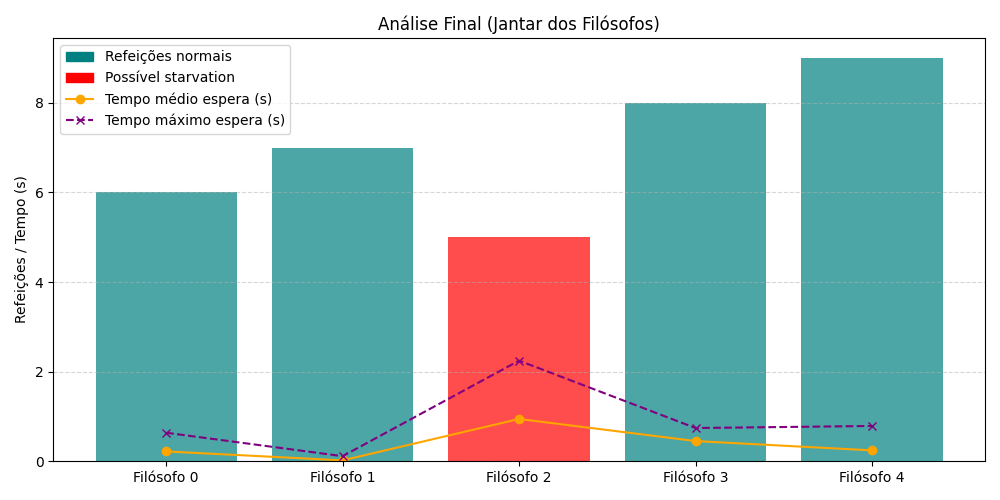
\includegraphics[width=0.7\textwidth]{images/analise_final.png}
    \caption{Distribuição de refeições, tempo médio e máximo de espera e possíveis starvations.}
\end{figure}

\section{Discussão}
Os resultados indicam que todos os filósofos conseguiram realizar um número semelhante de refeições ao longo da execução do algoritmo, evidenciando \textbf{equidade no acesso aos recursos}.  

O \textbf{tempo médio de espera} manteve-se baixo e estável, e o tempo máximo apresentou pequenas variações. Isso demonstra que o uso de \textit{mutex} minimizou contenções e garantiu fluidez no processo de alimentação.  

Não foram registradas situações de \textit{starvation} ou deadlock, reforçando a robustez da implementação.  

Comparando com soluções alternativas presentes na literatura, como algoritmos assimétricos ou baseados em semáforos, observa-se que abordagens menos restritivas podem aumentar a desigualdade de acesso e o tempo de espera, mostrando a eficácia do método adotado.

\section{Limitações}
Este estudo apresenta algumas limitações:

\begin{itemize}
    \item Apenas 5 filósofos simulados, limitando a generalização;
    \item Uso de threads Python, que não exploram paralelismo real de CPU devido ao GIL;
    \item Resultados dependem de tempos aleatórios de pensar e comer.
\end{itemize}

\section{Trabalhos Futuros}
Como possíveis extensões, sugerimos:

\begin{itemize}
    \item Avaliar diferentes algoritmos de sincronização (ex.: semáforos, monitores, soluções assimétricas);
    \item Simular cenários com maior número de filósofos e recursos para observar impacto na escalabilidade;
    \item Implementar versão distribuída em multiprocessos ou rede;
    \item Utilizar ferramentas de profiling para medir contenção e desempenho em tempo real.
\end{itemize}

\section{Conclusão}
A abordagem estatística aplicada ao problema do Jantar dos Filósofos permitiu avaliar de forma clara o comportamento do sistema.  

O algoritmo implementado garantiu:

\begin{itemize}
    \item Equidade no acesso aos recursos;
    \item Baixo tempo médio de espera;
    \item Ausência de starvation e deadlock.
\end{itemize}

O uso de \textit{locks} mostrou-se eficaz para resolver o problema de concorrência e demonstra a importância de técnicas de sincronização adequadas em sistemas multithread.

\section*{Referências}
\begin{itemize}
    \item Dijkstra, E. W. (1965). Solution of a problem in concurrent programming control.
\end{itemize}

\end{document}
